\chapter{Erstellung Orthofoto und Oberflächenmodell}

\label{ch:eval-aerial}

%----------------------------------------------------------------------------------------

\section{Wahl des Test-Objekts}

Zum Testen der Orthofoto- und Oberflächenmodell-Erstellung verschiedener
Softwarelösungen haben wir uns für das HSR Gelände entschieden. Am Tag der
Luftaufnahmen waren zudem Aufbauarbeiten für das Seenachtsfest in Gange, daher
sieht man auch einige Hüpfburgen und Zelte auf den Luftbildern.

Die Erfassung der Bilder wurde bereits im \autoref{workflow:hsr:drone}
beschrieben. Alle Bilder wurden mit GNSS-Koordinaten versehen.

Das resultierende Dataset enthält 124 Bilder, gesamthaft 1.2 GiB.

\begin{figure}[H]
	\centering
	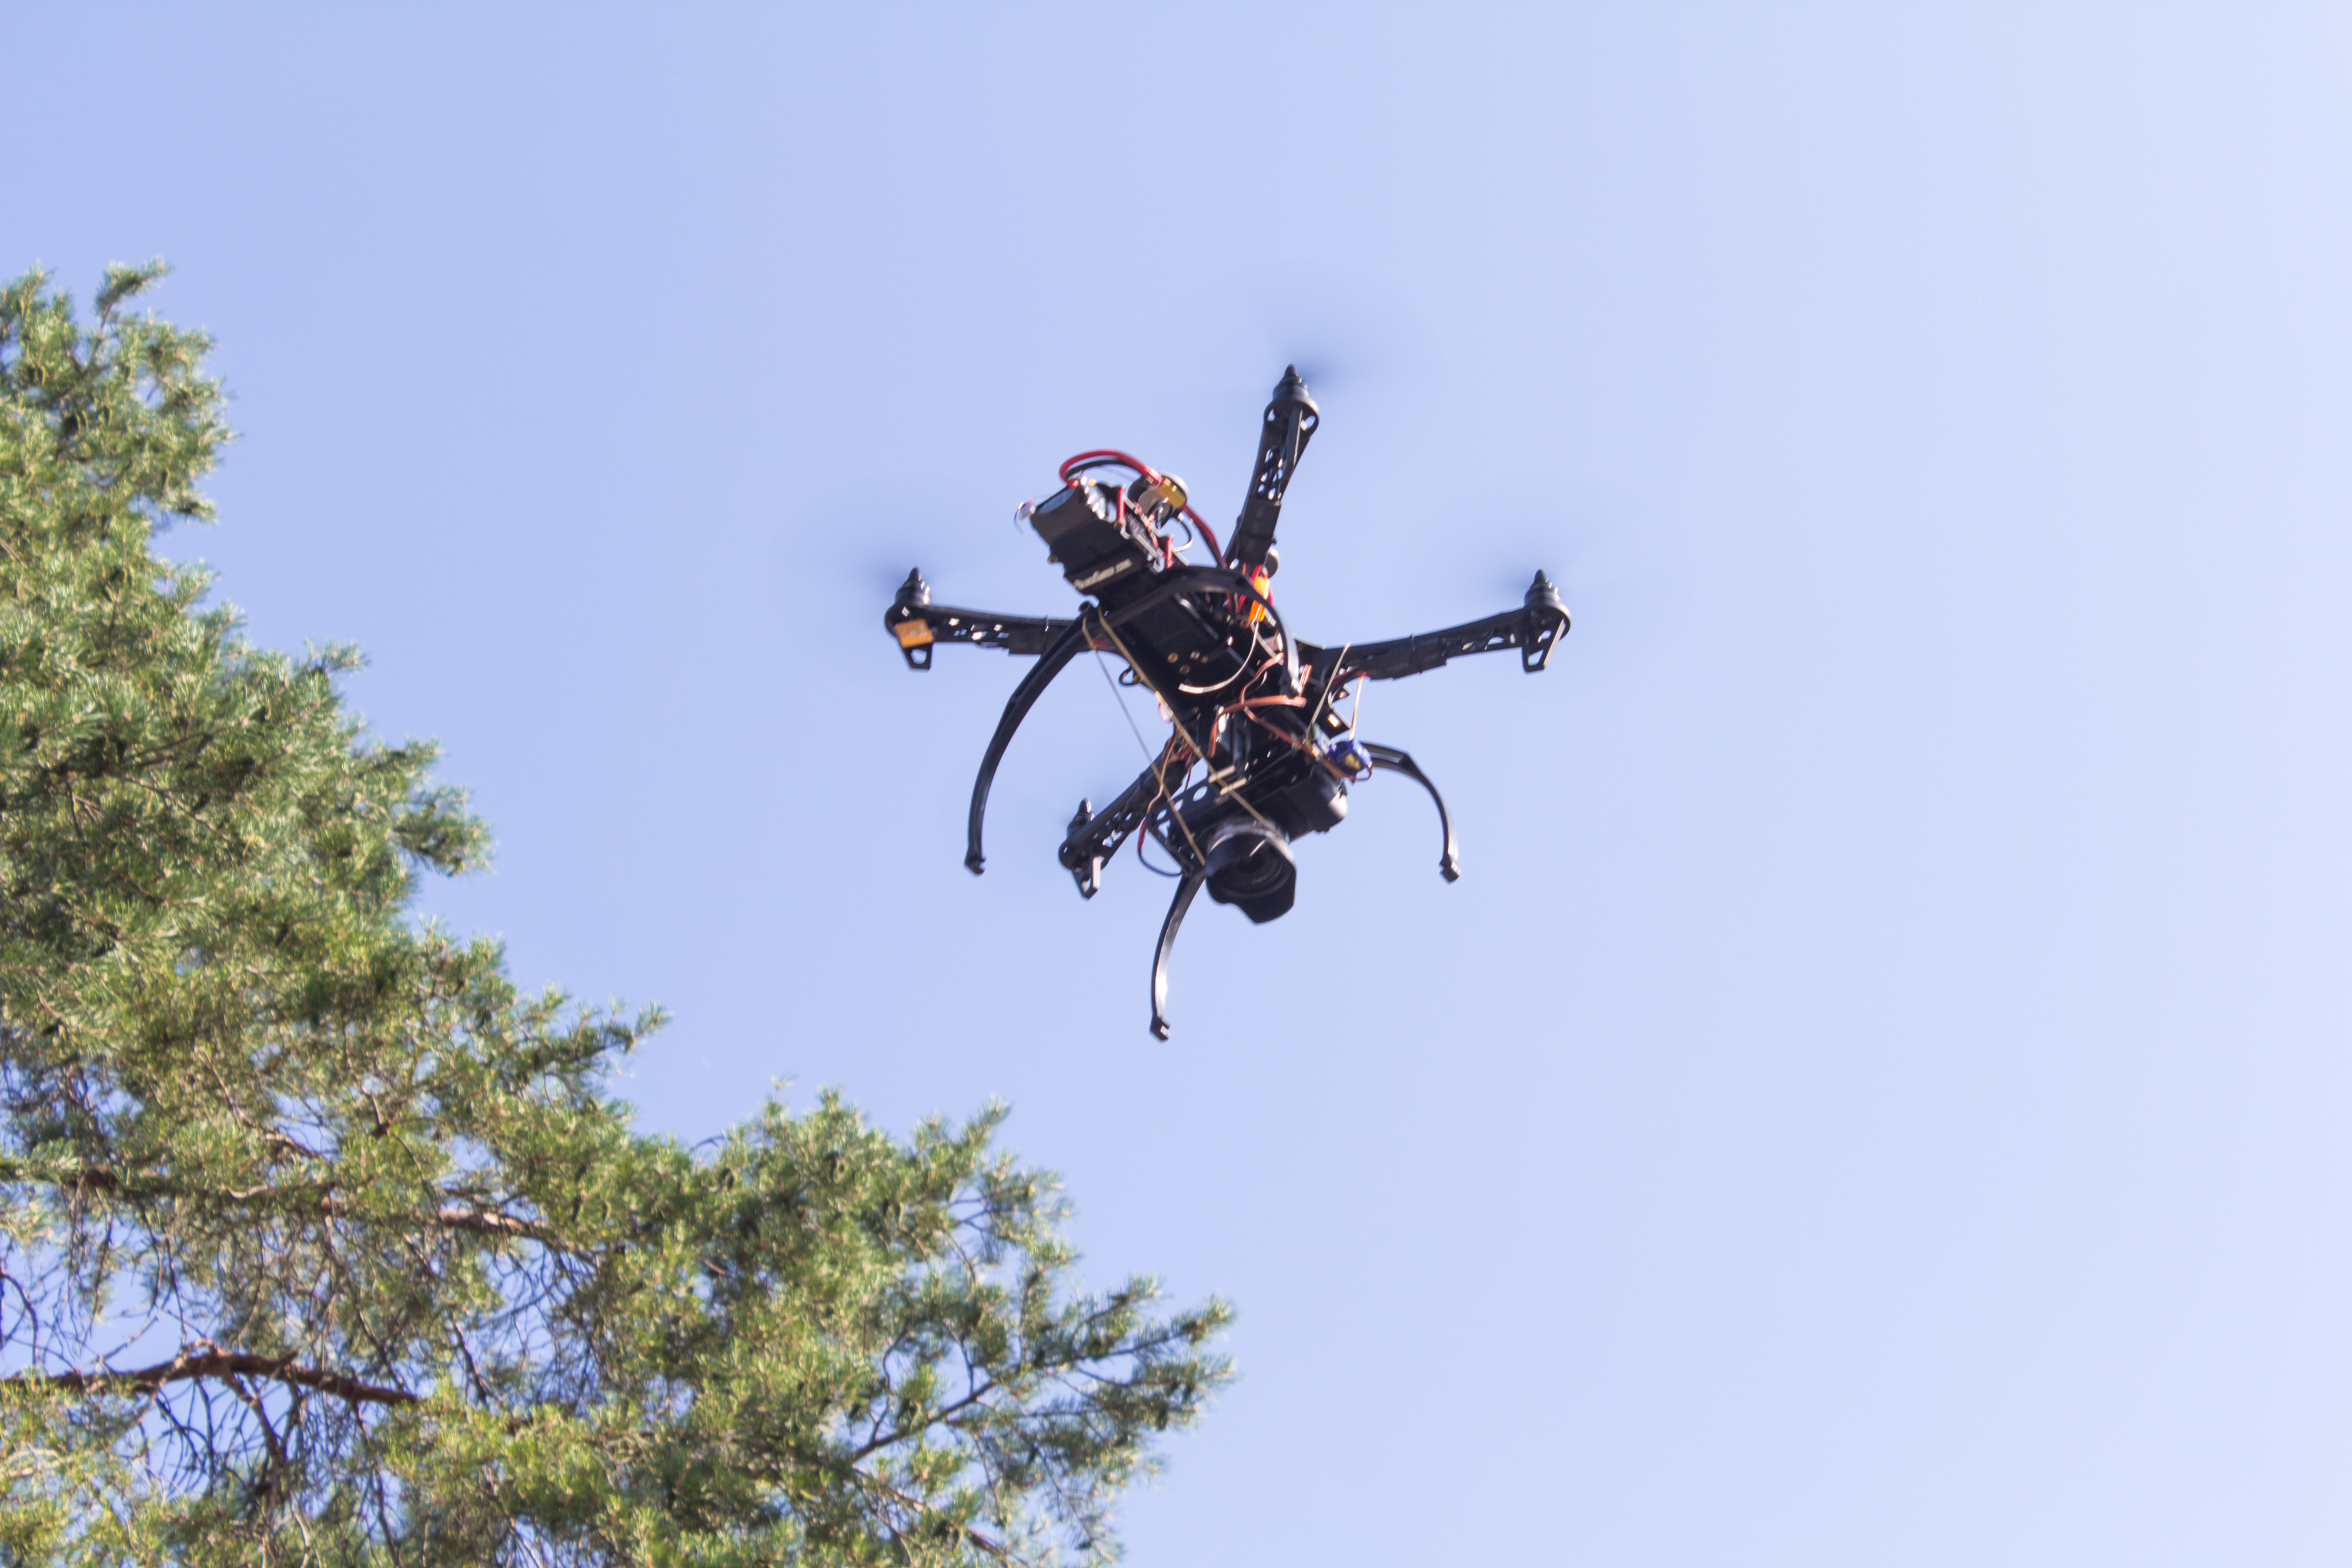
\includegraphics[width=\textwidth]{images/copter4.jpg}
	\caption{Erfassung Bildmaterial HSR}
	\label{img:copter4}
\end{figure}

%----------------------------------------------------------------------------------------

\newpage
\section{Resultate}

\subsection{Rekonstruktionsdauer}

Folgende Tabelle vergleicht die Rekonstruktionsdauer für das Oberflächenmodell
und für das Orthofoto.

\begin{figure}[H]
	\begin{tabularx}{\textwidth}[H]{Xccc}
		\toprule
		\textbf{Software} & \textbf{DSM + Orthofoto} \\
		\midrule
		OpenDroneMap & 2h 54min \\
		Pix4Dmapper Pro & 11h 16min \\
		PhotoScan Pro & 4h 56min \\
		\bottomrule
	\end{tabularx}
\end{figure}

\subsection{Komplexität der Resultate}

Als Vergleichsmass für die Komplexität der Resultate haben wir die Anzahl der
Pixel im Orthofoto sowie die Anzahl der Vertizes im Oberflächenmodell verwendet.

Dies ist natürlich nur bedingt aussagekräftig, da die Anzahl der Pixel bzw.
Vertizes von den Konversions-Parametern abhängig ist und auch nicht zwingend
etwas über die Qualität des Bildes bzw. Modells aussagt.

\begin{figure}[H]
	\begin{tabularx}{\textwidth}[H]{Xcc}
		\toprule
		\textbf{Software} & \textbf{Pixel in Orthofoto} & \textbf{Vertizes in DSM} \\
		\midrule
		OpenDroneMap & 10'112 x 9'066 & 100'050 \\
		Pix4Dmapper Pro & 20'772 x 15'988 & 498'202 \\
		PhotoScan Pro & 23'254 x 19'496 & 685'956 \\
		\bottomrule
	\end{tabularx}
\end{figure}

%----------------------------------------------------------------------------------------

\begin{figure}[p]
	\centerline{
		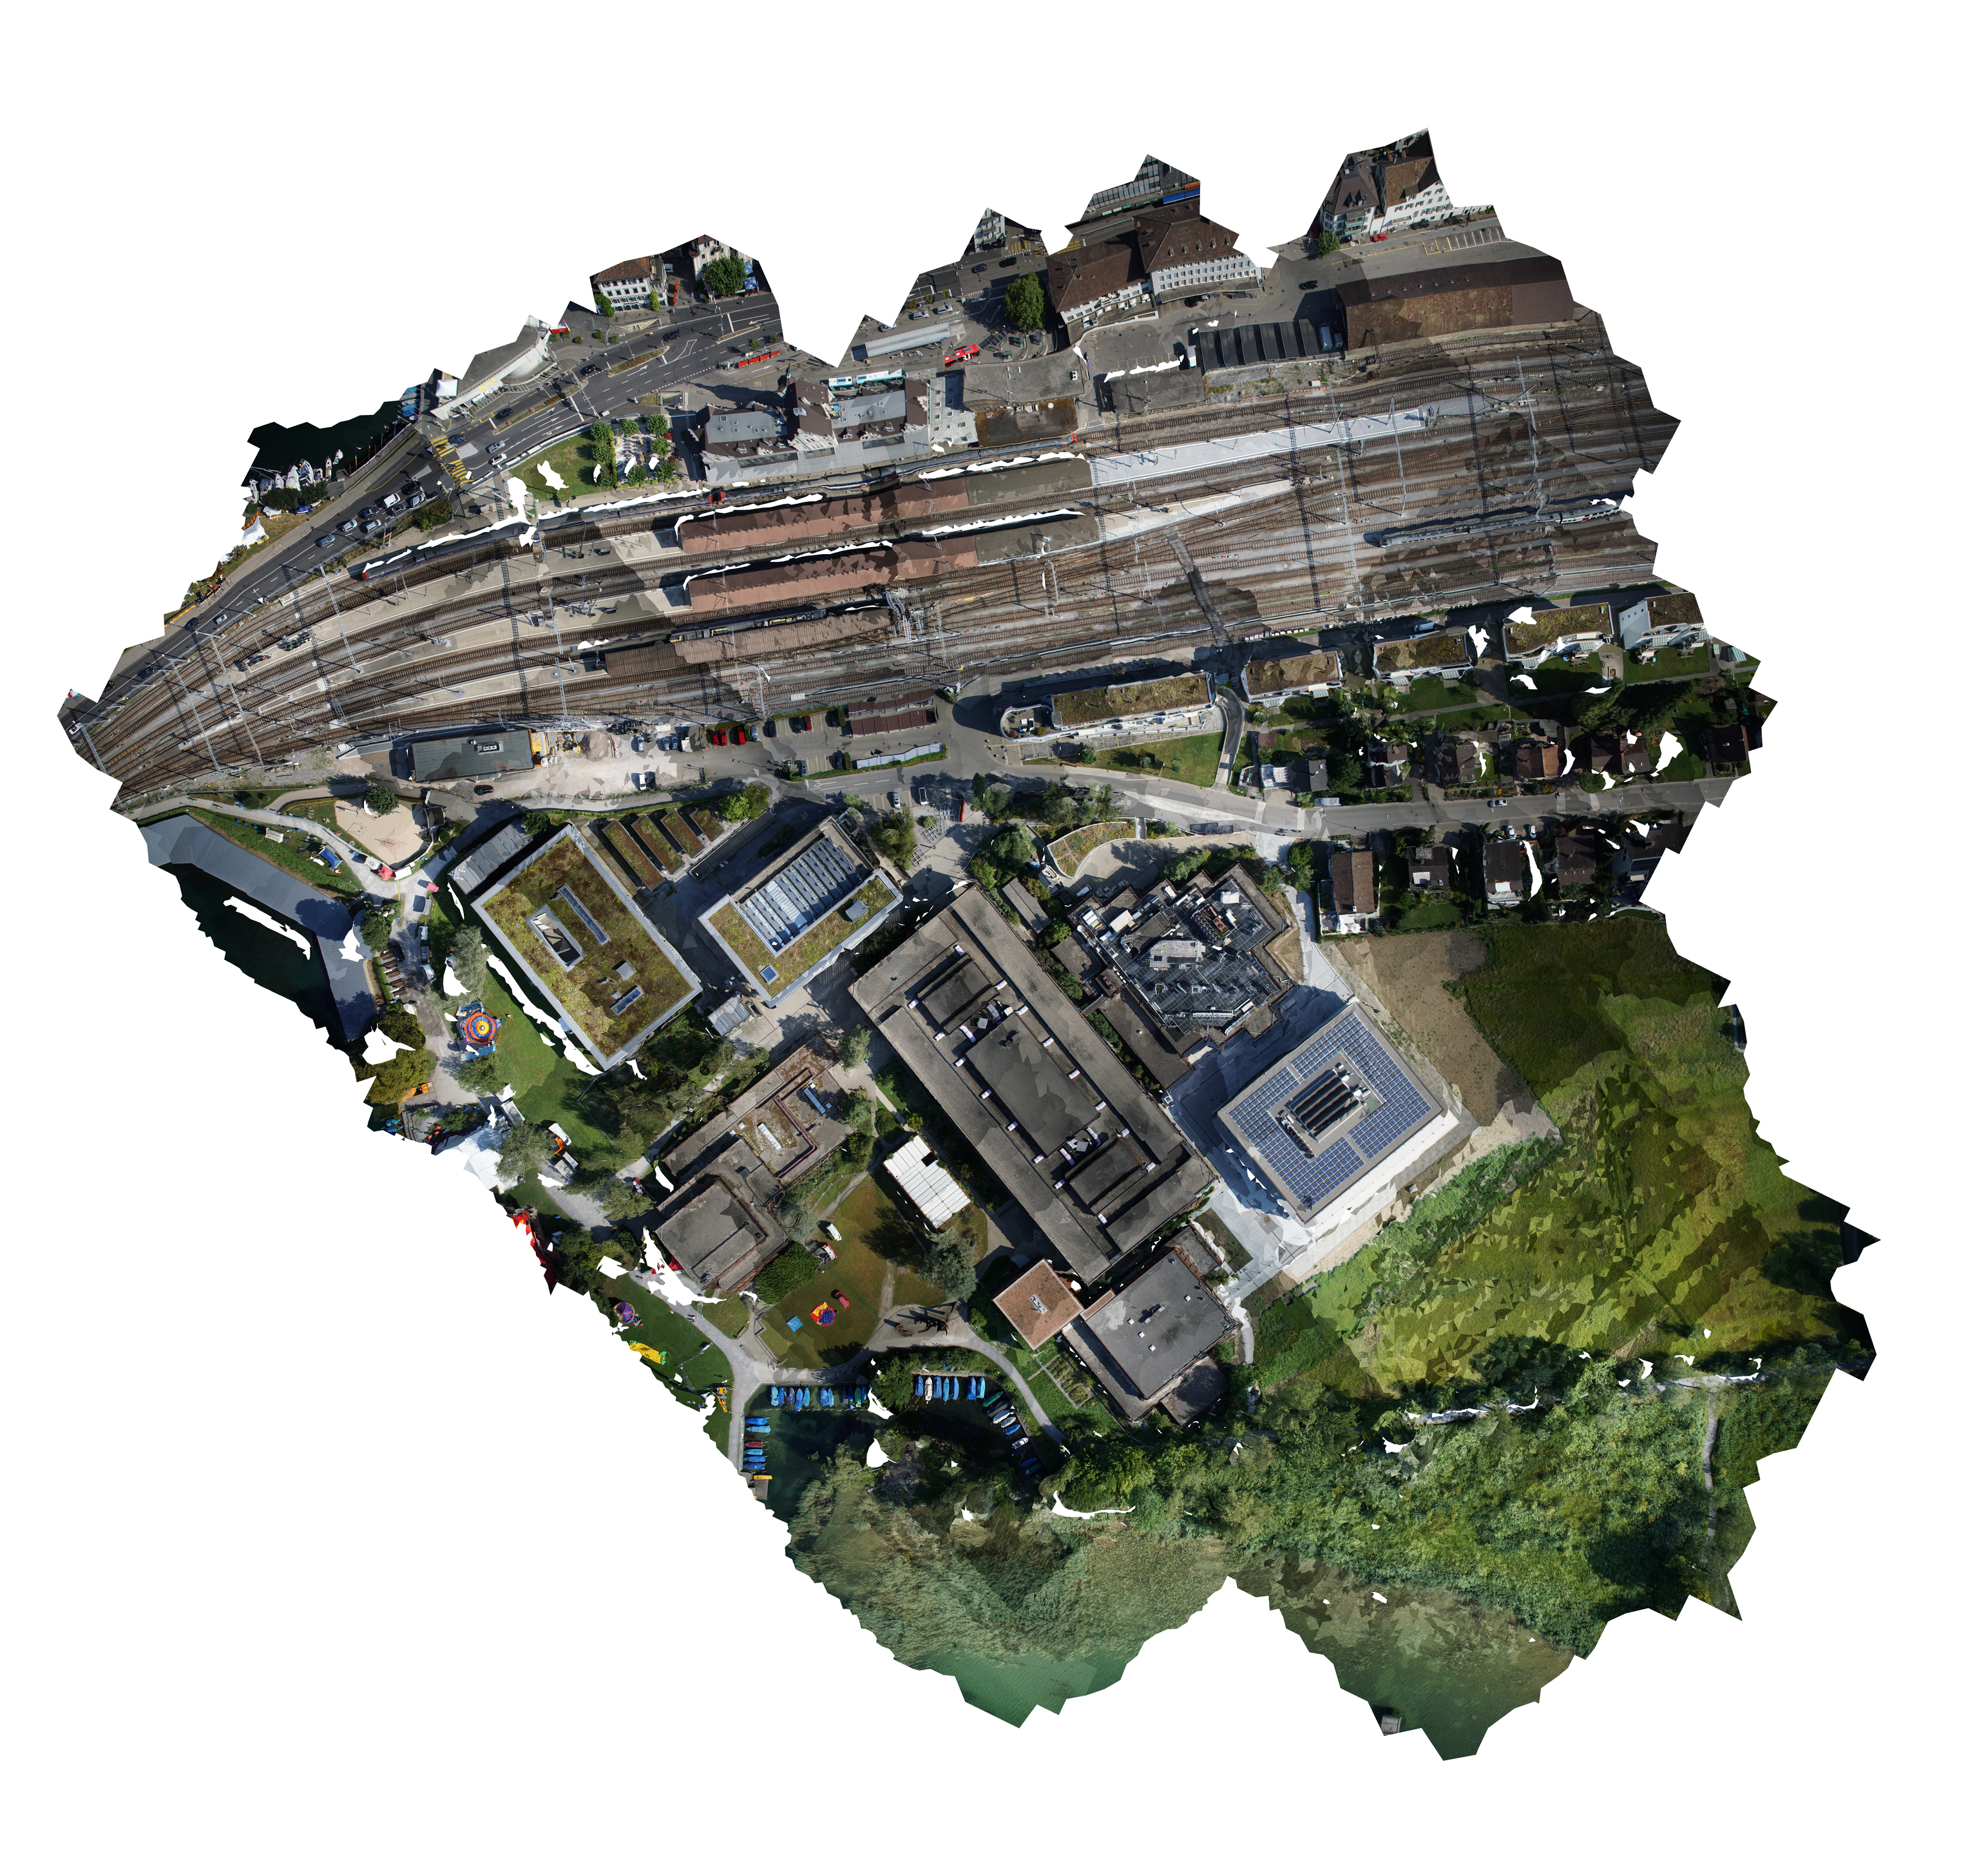
\includegraphics[width=16cm]{images/hsr-ortho-odm.png}
	}
	\caption{Resultat: Orthofoto HSR mit OpenDroneMap}
	\label{img:hsr-ortho-odm}
\end{figure}

\begin{figure}[p]
	\centerline{
		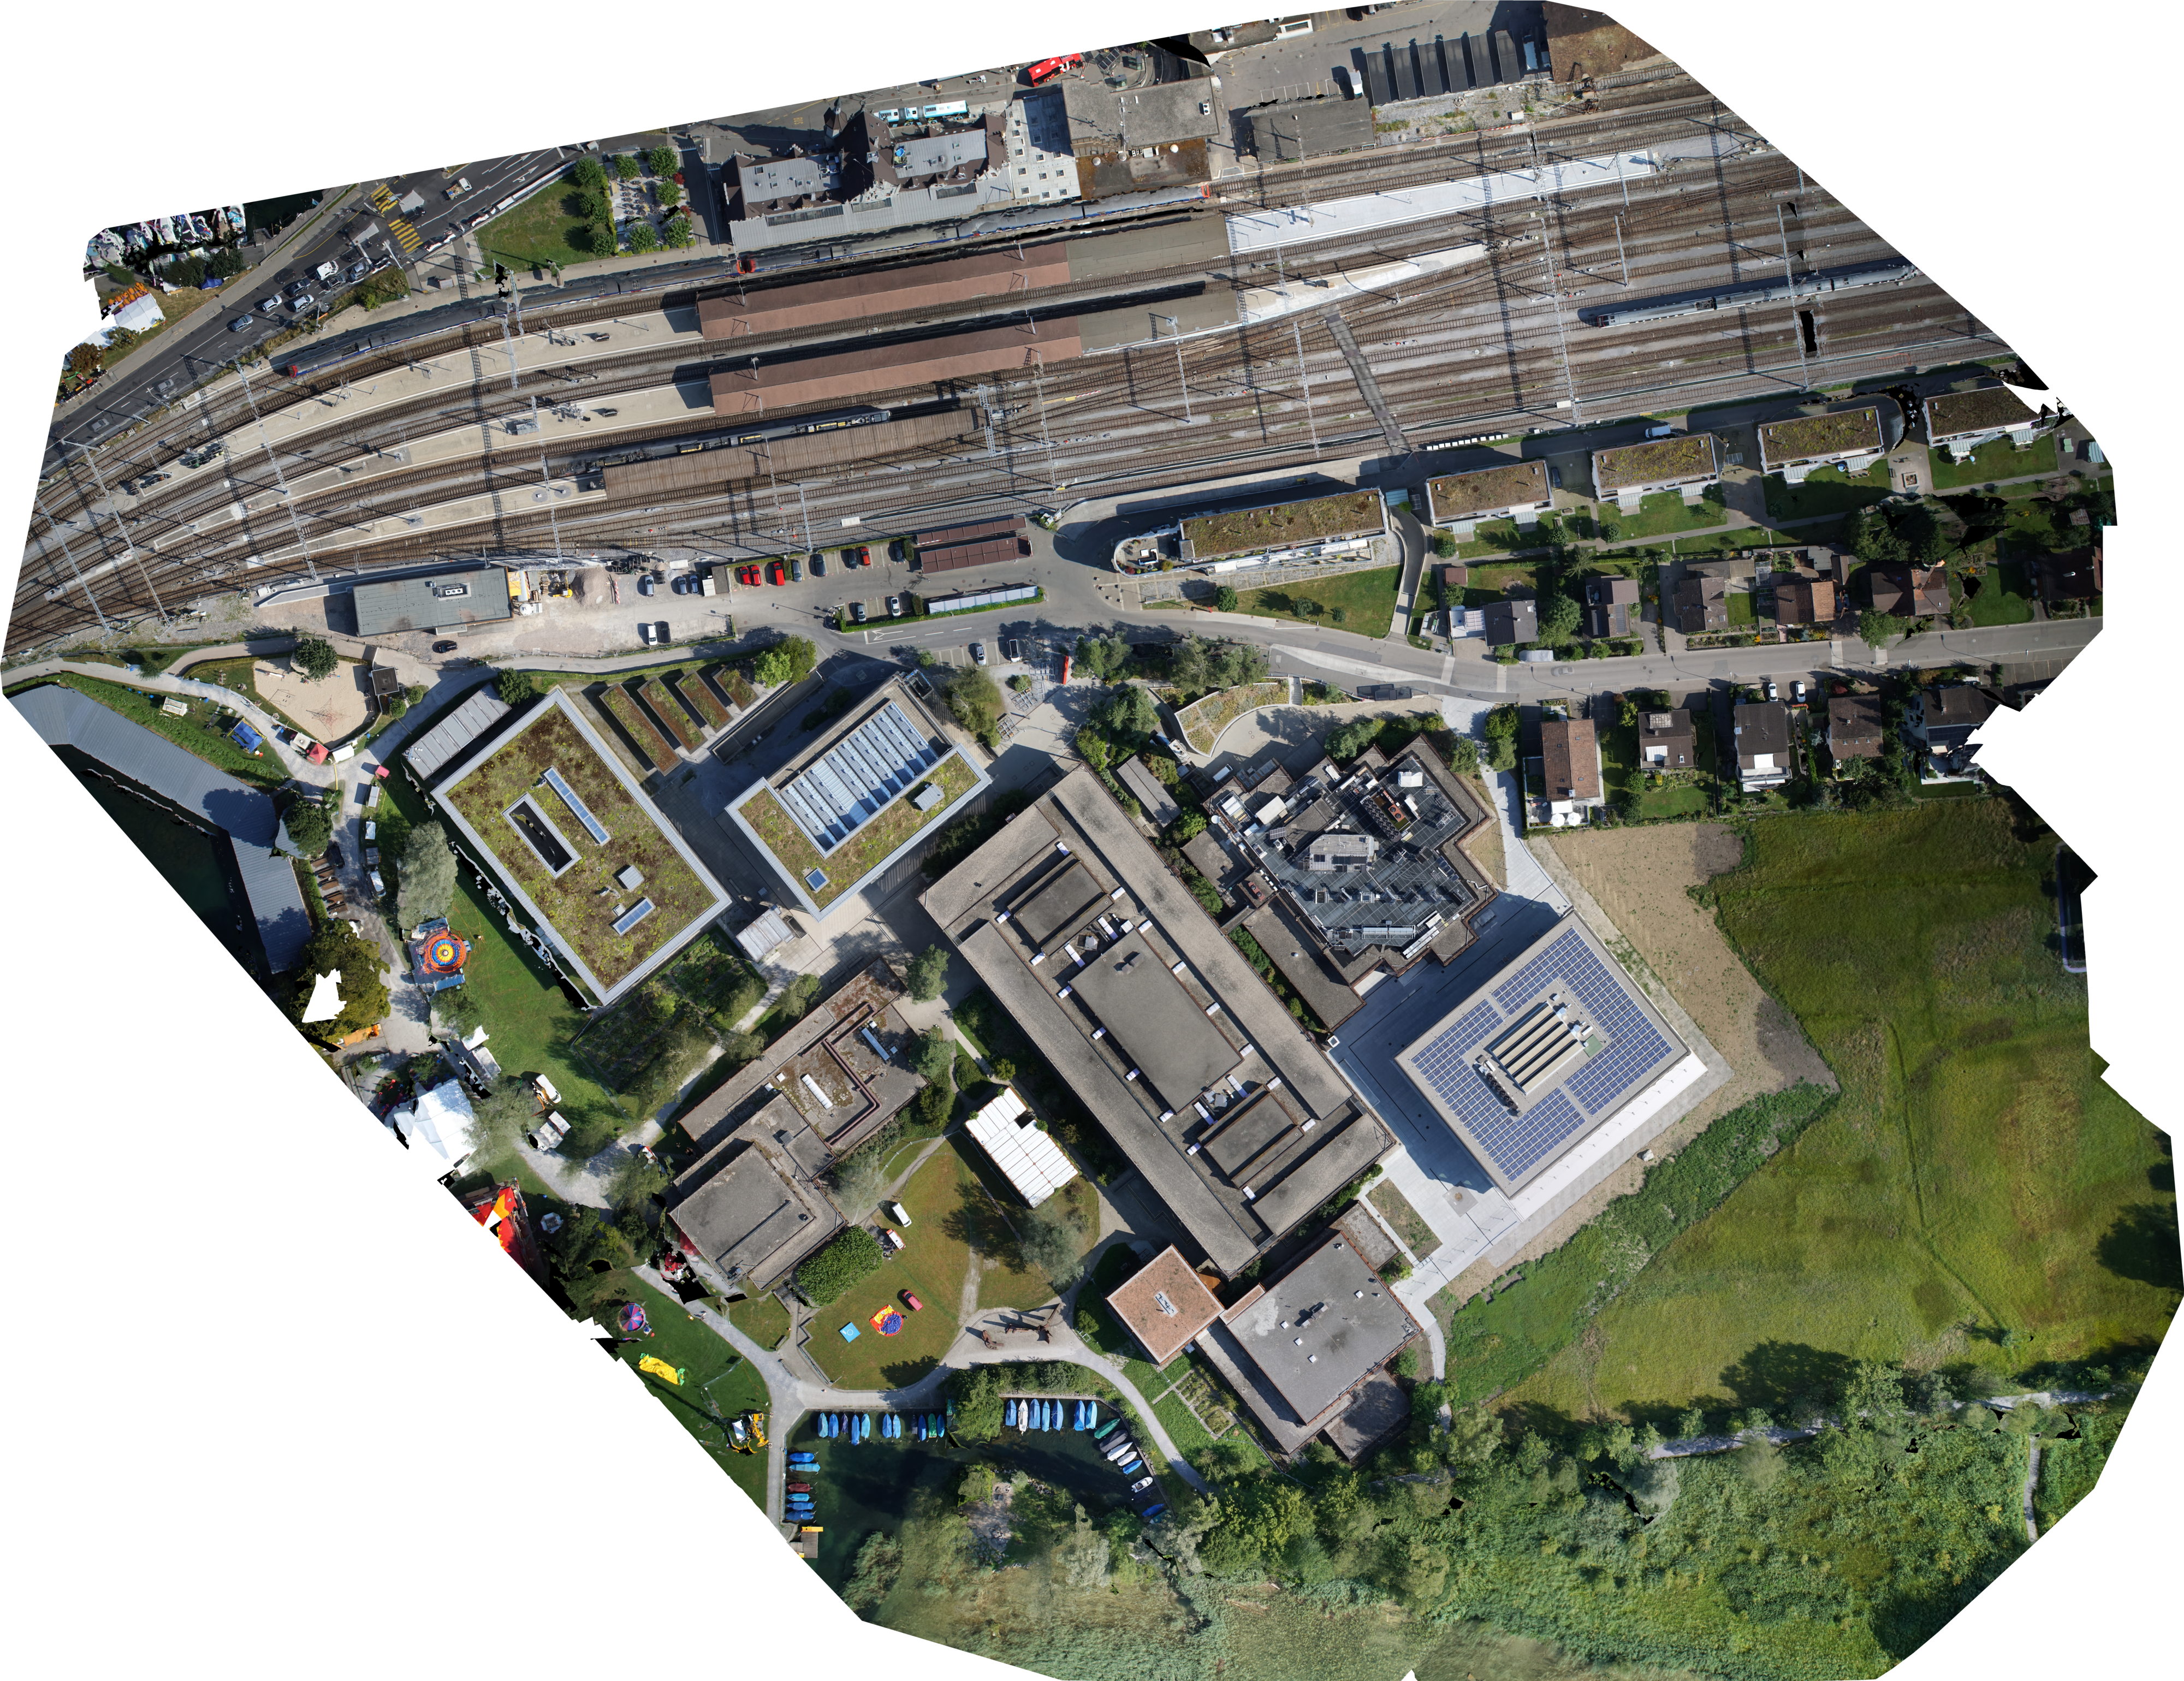
\includegraphics[width=15cm]{images/hsr-ortho-pix4d.png}
	}
	\caption{Resultat: Orthofoto HSR mit Pix4Dmapper Pro}
	\label{img:hsr-ortho-pix4d}
\end{figure}

\begin{figure}[p]
	\centerline{
		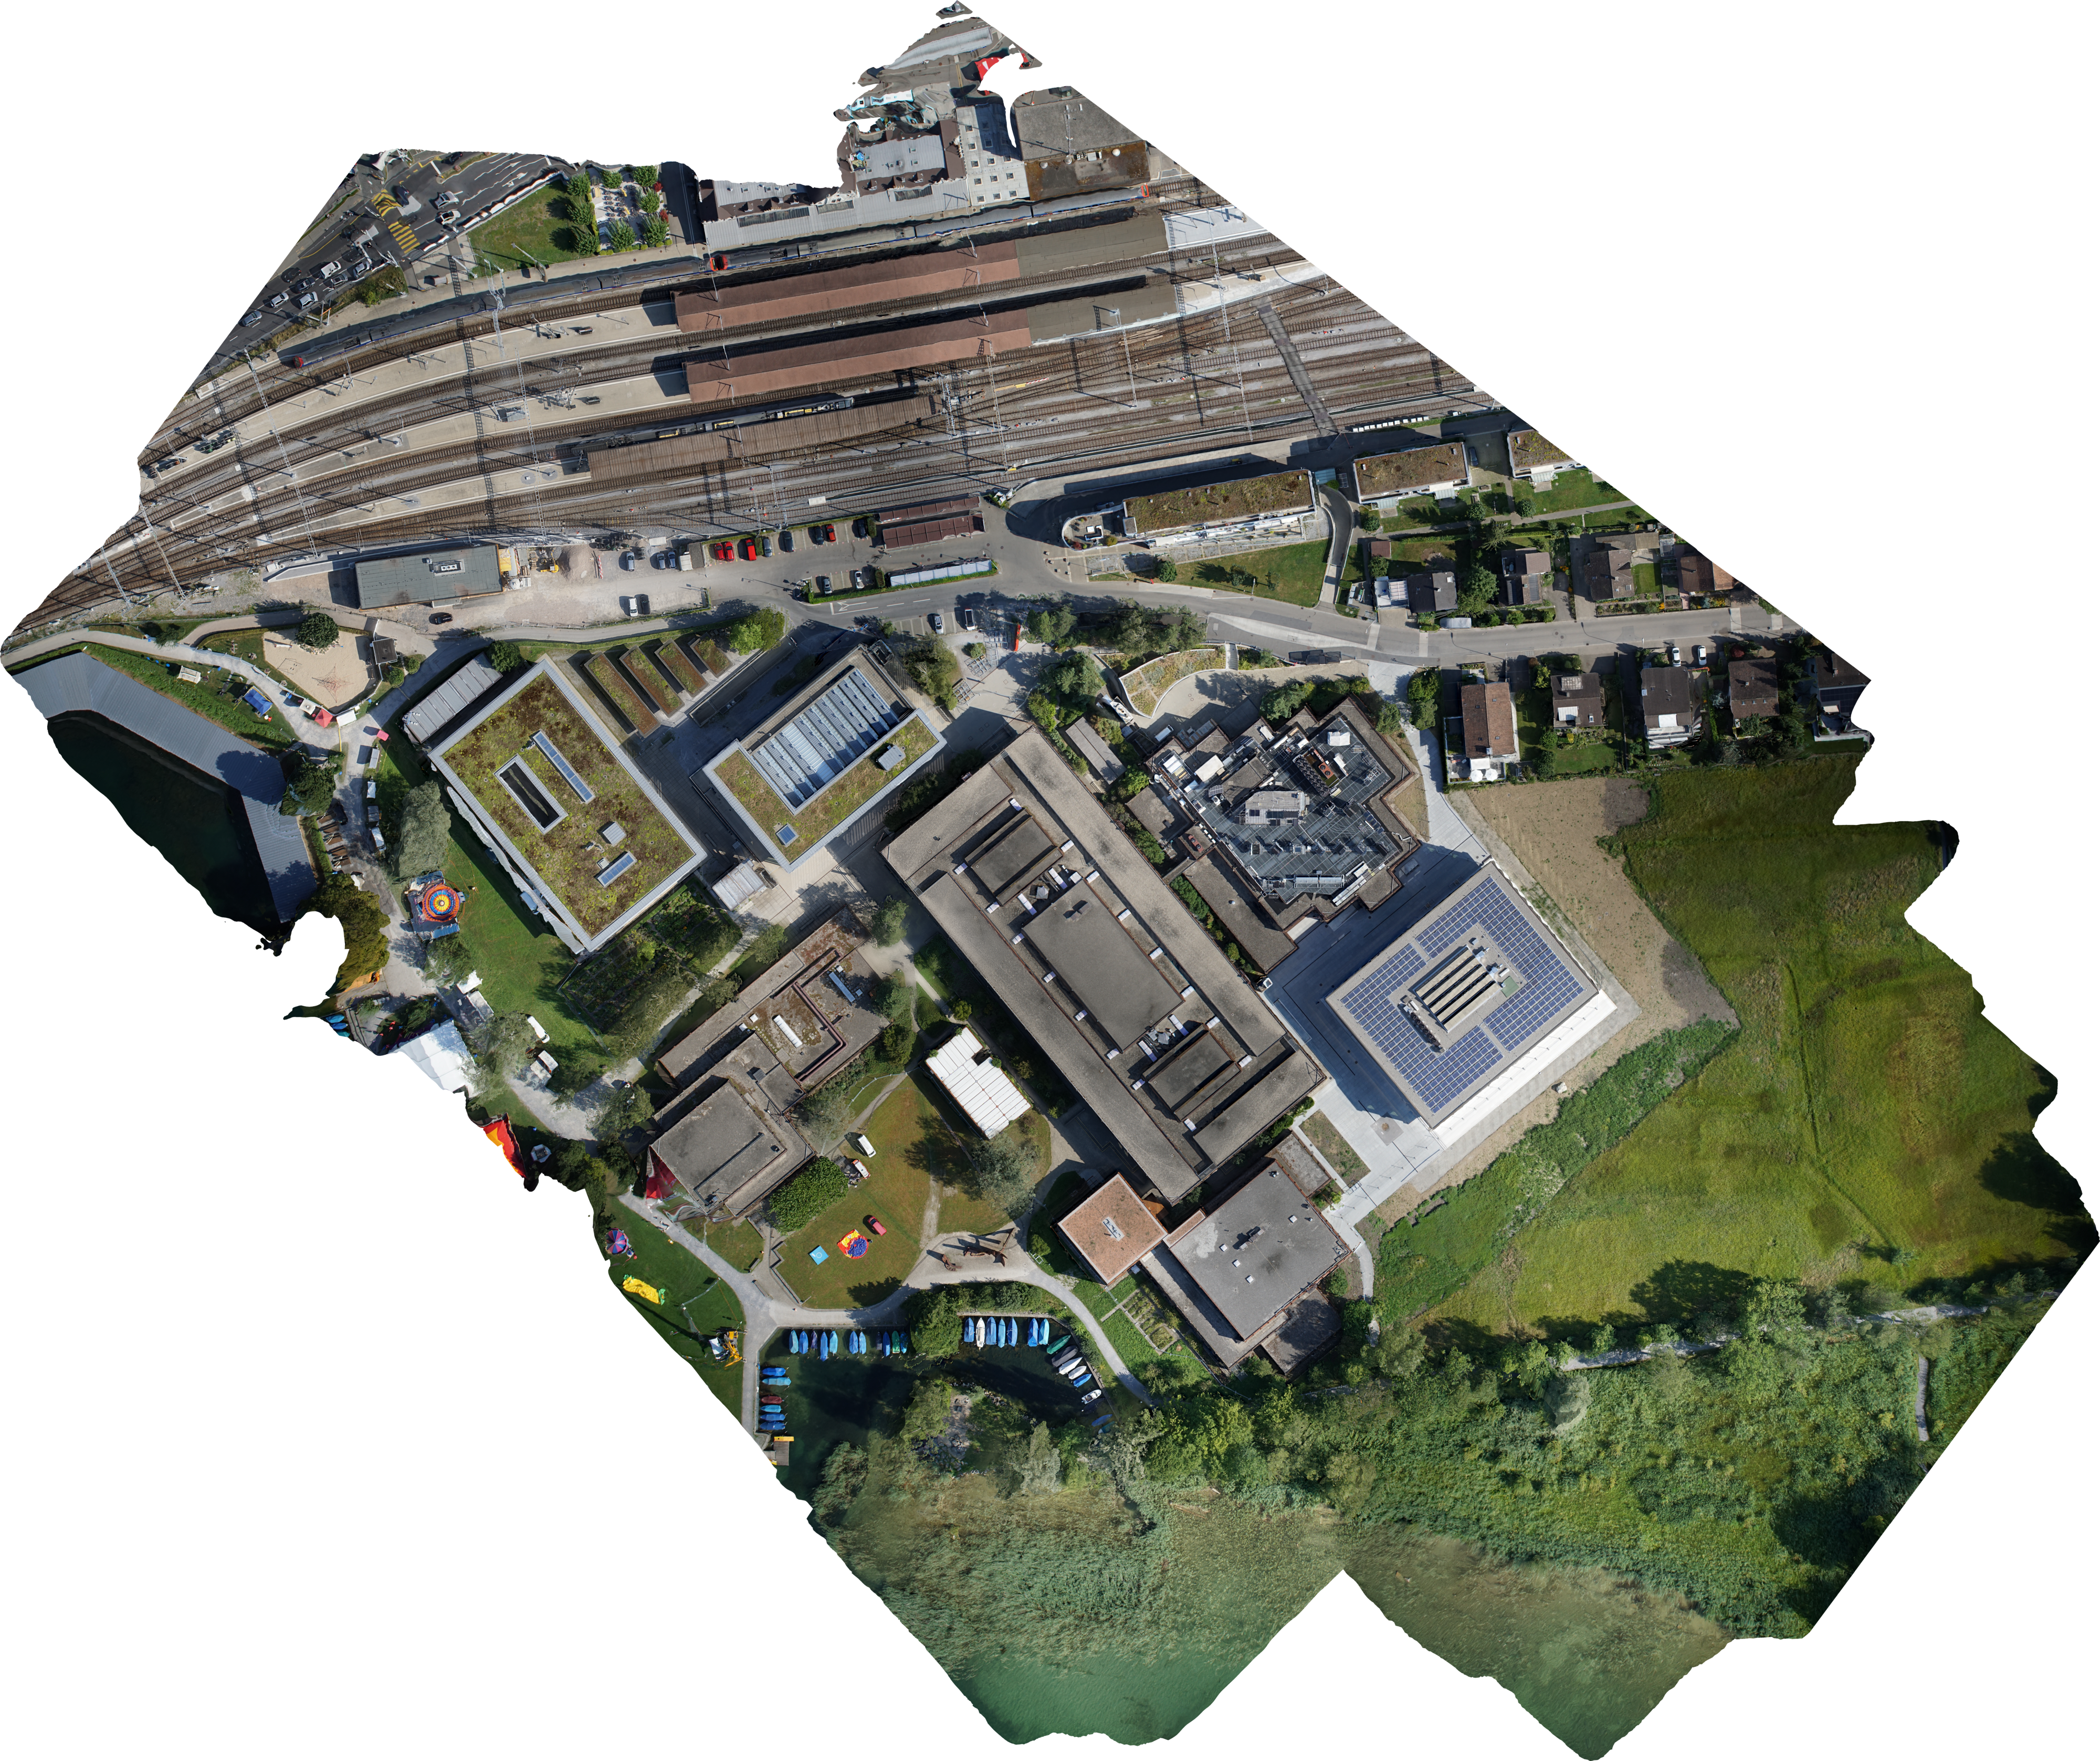
\includegraphics[width=15cm]{images/hsr-ortho-photoscan.png}
	}
	\caption{Resultat: Orthofoto HSR mit PhotoScan Pro}
	\label{img:hsr-ortho-pix4d}
\end{figure}

%----------------------------------------------------------------------------------------

\begin{figure}[p]
	\centerline{
		\includegraphics[width=16cm]{images/hsr-dsm-odm.png}
	}
	\caption{Resultat: Oberflächenmodell HSR mit OpenDroneMap}
	\label{img:hsr-dsm-odm}
\end{figure}

\begin{figure}[p]
	\centerline{
		\includegraphics[width=15cm]{images/hsr-dsm-pix4d.png}
	}
	\caption{Resultat: Oberflächenmodell HSR mit Pix4Dmapper Pro}
	\label{img:hsr-dsm-pix4d}
\end{figure}

\begin{figure}[p]
	\centerline{
		\includegraphics[width=15cm]{images/hsr-dsm-photoscan.png}
	}
	\caption{Resultat: Oberflächenmodell HSR mit PhotoScan Pro}
	\label{img:hsr-dsm-pix4d}
\end{figure}

%----------------------------------------------------------------------------------------
